\documentclass[english]{beamer}
\usepackage[T1]{fontenc}
\usepackage[latin9]{inputenc}
\setcounter{secnumdepth}{3}
\setcounter{tocdepth}{3}
\usepackage{amssymb}
\usepackage{stmaryrd}
\usepackage{alltt}
\usepackage{mathpartir}
\usepackage{url}
\usepackage{bussproofs}
\usepackage{ulem} % for xout, sout
\usepackage{ae}
\usepackage{tikz}
\usetikzlibrary{snakes}
\usetikzlibrary{arrows}
\usetikzlibrary{shapes}

\usepackage{babel}

\frenchspacing

\begin{document}

\title{Parametricity, Quotient Types, \\ and Theorem Transfer}
\author{Brian Huffman}
%\author{Brian Huffman \\ \medskip \small{based on joint work with Ond\v{r}ej Kun\v{c}ar, T.U. Munich}}
%\institute{Technische Universit\"at M\"unchen}
\institute{Galois Tech Seminar}
\date{March 5, 2013}

\begin{frame}
\titlepage
\end{frame}


\begin{frame}
\frametitle{Outline}

\begin{large}
\begin{enumerate}[I]
\item Parametricity, free theorems
\medskip
\item Quotient types, subtypes (type abstraction)
\medskip
\item Theorem transfer, Isabelle/HOL automation
\end{enumerate}
\end{large}

\end{frame}

\section{Parametricity}
\begin{frame}
\begin{center}
\huge{Parametricity}
\end{center}
\end{frame}

\begin{frame}
\frametitle{Parametricity}
Parametrically polymorphic functions
\begin{itemize}
\item may be instantated at different types
\item all instances behave uniformly
\item limited in what they can do with their arguments
\end{itemize}
\bigskip
How to make this precise?
\end{frame}

\begin{frame}
\frametitle{Idea: Types as Relations}
Mapping $\llbracket - \rrbracket$ takes type expressions to binary relations \\
\bigskip
\pause
Ground types are identity relations
\begin{itemize}
\item $\llbracket \mathtt{Int} \rrbracket = \mathit{Id}_\mathtt{Int}$
\item $\llbracket \mathtt{Bool} \rrbracket = \mathit{Id}_\mathtt{Bool}$
\end{itemize}
\bigskip
\pause
Functions are related if they take related input to related output
\begin{itemize}
\item $\llbracket \tau_1 \to \tau_2 \rrbracket = \llbracket\tau_1\rrbracket \Mapsto \llbracket\tau_2\rrbracket$
\item $(A \Mapsto B)\:f\:g \Longleftrightarrow (\forall x\,y.\:A\:x\:y \implies B\:(f\:x)\:(g\:y))$
\end{itemize}
\bigskip
\pause
Type variables map to arbitrary relations
\begin{itemize}
\item $\llbracket \mathtt{a} \rrbracket = A$
\item $\llbracket \mathtt{b} \rrbracket = B$
\end{itemize}
\end{frame}

\begin{frame}
\frametitle{The Parametricity Theorem}
\textbf{Theorem.} If term $f$ has type $\tau$, then $\llbracket\tau\rrbracket\:f\:f$\\
\bigskip
\pause
Example:
\begin{itemize}
\item $\mathtt{foo} :: \mathtt{a} \to \mathtt{b} \to \mathtt{a}$
\item $\llbracket \mathtt{a} \to \mathtt{b} \to \mathtt{a} \rrbracket\;\mathtt{foo}\;\mathtt{foo}$
\item $(A \Mapsto B \Mapsto A)\;\mathtt{foo}\;\mathtt{foo}$ (for arbitrary $A, B$)
\item $A\:x\:x' \land B\:y\:y' \implies A\:(\mathtt{foo}\:x\:y)\:(\mathtt{foo}\:x'\:y')$
\item Implies e.g.\ that $\mathtt{foo}\:x\:y = x$
\end{itemize}
\end{frame}

\begin{frame}
\frametitle{Proof of the Parametricity Theorem}
Lambda calculus typing rules:
\begin{mathpar}
\inferrule*[Right=App]
{\Gamma \vdash f : \tau_1 \to \tau_2 \\ \Gamma \vdash x : \tau_1}
{\Gamma \vdash f\:x : \tau_2}
\\
\inferrule*[Right=Abs]
{\Gamma, x : \tau_1 \vdash u : \tau_2}
{\Gamma \vdash \lambda x.\:u : \tau_1 \to \tau_2}
\and
\inferrule*[Right=Var]
{x : \tau \in \Gamma}
{\Gamma \vdash x : \tau}
\end{mathpar}
\pause
Inference rules for relations:
\begin{mathpar}
\inferrule*[Right=App]
{\Gamma \vdash (R_1 \Mapsto R_2)\:f\:g \\ \Gamma \vdash R_1\:x\:y}
{\Gamma \vdash R_2\:(f\:x)\:(g\:y)}
\\
\inferrule*[Right=Abs]
{\Gamma, R_1\:x\:y \vdash R_2\:u\:v}
{\Gamma\vdash (R_1 \Mapsto R_2)\:(\lambda x.\:u)\:(\lambda y.\:v)}
\and
\inferrule*[Right=Var]
{R\:x\:y \in \Gamma}
{\Gamma \vdash R\:x\:y}
\end{mathpar}
\end{frame}

\begin{frame}
\frametitle{Parametricity with Datatypes}
Data structures are related if
\begin{itemize}
\item they have the same shape
\item elements are related pointwise
\end{itemize}
\bigskip
\pause
Pairs
\begin{itemize}
%\item $\llbracket (\tau_1, \tau_2) \rrbracket = \llbracket \tau_1 \rrbracket \otimes \llbracket \tau_2 \rrbracket$
\item $(A \otimes B)\:(x, y)\:(x', y') \Longleftrightarrow A\:x\:x' \land B\:y\:y'$
%\item $(A \Mapsto B \Mapsto A \otimes B)\:(,)\:(,)$
\end{itemize}
\medskip
Lists
\begin{itemize}
%\item $\llbracket \mathtt{[}\tau\mathtt{]} \rrbracket = \llbracket \tau \rrbracket ^{*}$
\item $A^{*}\:\mathtt{[\:]}\:{[\:]}$
\item $A^{*}\:(x : xs)\:(x' : xs') \Longleftrightarrow A\:x\:x' \land A^{*}\:xs\:xs'$
%\item $(A \Mapsto A^{*} \Mapsto A^{*})\:(:)\:(:)$
\end{itemize}
\medskip
Constructors satisfy parametricity theorem
\begin{itemize}
\item $(A \Mapsto B \Mapsto A \otimes B)\:(,)\:(,)$
%$(,) :: \mathtt{a} \to \mathtt{b} \to (\mathtt{a},\mathtt{b})$
\item $(A \Mapsto A^{*} \Mapsto A^{*})\:(:)\:(:)$
% $(:) :: \mathtt{a} \to [\mathtt{a}] \to [\mathtt{a}]$
\end{itemize}
\end{frame}

\begin{frame}
\frametitle{Theorems for Free! (Wadler)}
Recipe for generating free theorems:
\begin{enumerate}
\item Start with parametricity theorem for the given type
\item Instantiate relations with graphs of functions
\item Simplify
\end{enumerate}
\bigskip
\pause
Example:
\begin{itemize}
\item $\mathtt{reverse} :: [\mathtt{a}] \to [\mathtt{a}]$
\item $(A^{*} \Mapsto A^{*})\:\mathtt{reverse}\:\mathtt{reverse}$
\item Let $A = \mathit{graph}(f)$
\item Then $A^{*} = \mathit{graph}(\mathtt{map}\:f)$
\item $A^{*}\:xs\:ys \implies A^{*}\:(\mathtt{reverse}\:xs)\:(\mathtt{reverse}\:ys)$
\item $\mathtt{map}\:f\:xs = ys \implies \mathtt{map}\:f\:(\mathtt{reverse}\:xs) = \mathtt{reverse}\:ys$
\item $\mathtt{map}\:f\:(\mathtt{reverse}\:xs) = \mathtt{reverse}\:(\mathtt{map}\:f\:xs)$
\end{itemize}
\end{frame}

\begin{frame}
\frametitle{Not-Quite-Parametric Functions}
Some functions are polymorphic, but not completely parametric
\\
\bigskip
\begin{overlayarea}{\textwidth}{6cm}
\only<2-3>{
Example:
\begin{itemize}
\item $(=) :: \mathtt{a} \to \mathtt{a} \to \mathtt{Bool}$
\item Its type suggests $(A \Mapsto A \Mapsto \mathit{Id}_\mathtt{Bool})\:(=)\:(=)$
\item I.e.\ $A\:x\:x' \land A\:y\:y' \implies (x = y \Longleftrightarrow x' = y')$
\end{itemize}
}
\only<3>{
\bigskip
Not true for all $A$, but for some $A$
\begin{itemize}
\item Valid iff $A$ is single-valued in both directions (bi-unique)
\item $\mathit{bi\textit{-}unique}(A) \implies (A \Mapsto A \Mapsto \mathit{Id}_\mathtt{Bool})\:(=)\:(=)$
%\item $\mathit{bi\textit{-}unique}(A) \approx \mathtt{Eq}\:\mathtt{a}$
\item Extra assumption works like \texttt{Eq} constraint
\end{itemize}
}
\only<4>{
Example 2:
\begin{itemize}
\item $(\forall) :: (\mathtt{a} \to \mathtt{Bool}) \to \mathtt{Bool}$
\item Its type suggests $((A \Mapsto \mathit{Id}_\mathtt{Bool}) \Mapsto \mathit{Id}_\mathtt{Bool})\:(\forall)\:(\forall)$
\item I.e.\ $(\forall x\,y.\:A\:x\:y \implies p\:x \Leftrightarrow q\:y) \implies (\forall x.\:p\:x) \Leftrightarrow (\forall y.\:q\:y)$
\end{itemize}
}
\only<4>{
\bigskip
Not true for all $A$, but for some $A$
\begin{itemize}
\item Valid iff $A$ is surjective in both directions (bi-total)
\item $\mathit{bi\textit{-}total}(A) \implies ((A \Mapsto \mathit{Id}_\mathtt{Bool}) \Mapsto \mathit{Id}_\mathtt{Bool})\:(\forall)\:(\forall)$
\item Extra assumption works like a class constraint
\end{itemize}
}
\end{overlayarea}
\end{frame}

\begin{frame}
\frametitle{Parametricity in Higher Order Logic}
{\large{Theorems for \xout{free} cheap!}}\\
\bigskip
Non-parametric polymorphic functions exist ($=, \forall$)
\begin{itemize}
\item Can't infer theorems from types alone
\item Must prove parametricity theorem for each constant
\item Easy syntax-directed proof (App/Abs/Var rules)
\item Some constants need $\mathit{bi\textit{-}unique}$ or $\mathit{bi\textit{-}total}$ constraints
\end{itemize}
\end{frame}

\begin{frame}
\frametitle{Parametricity in Higher Order Logic}
Isabelle/HOL maintains a database of parametricity theorems
\medskip
\begin{itemize}
\item Wadler-style free theorems are one application
\end{itemize}
\bigskip
How else can we use parametricity?
\end{frame}


\section{Quotient Types}
\begin{frame}
\begin{center}
\huge{Quotient Types}
\end{center}
\end{frame}

\begin{frame}
\frametitle{Quotients and subtypes are everywhere}
\begin{itemize}
\item integers
\item rationals
\item reals
\item n-bit words
\item multisets
\item finite sets
\item finite maps
\item vectors $\mathbb{R}^n$
\item balanced trees
\item ...
\end{itemize}
\end{frame}

\begin{frame}
\frametitle{Quotients and subtypes are \textbf{type abstractions}}
Hidden details of type construction and representation\\
\bigskip
Properties encoded in type signatures
\begin{itemize}
\item functions maintain datatype invariant
\item functions respect equivalence relation
\end{itemize}
\bigskip
Equality on abstract type $\longleftrightarrow$ other relation on raw type
\end{frame}

\begin{frame}[fragile]
\frametitle{Formalizing a new abstract type}
\begin{enumerate}
\item Define representation (``raw'') type
\item Define raw operations
\item Prove theorems about raw operations
\item Construct abstract type
\item \textbf{Lift operations} from raw to abstract
\item \textbf{Transfer theorems} from raw to abstract
\end{enumerate}
\end{frame}

\begin{frame}
\frametitle{Example: Quotient construction of $\mathbb{Z}$}

\begin{enumerate}[<+->]
\item Raw type: $\mathbb{N} \times \mathbb{N}$
\item Raw operation: $(x, y) +_\mathtt{raw} (u, v) = (x+u, y+v)$\\
  Raw operation: $(x, y) \le_\mathtt{raw} (u, v) = (x+v \le u+y)$\\
  Equivalence relation: $(x, y) \approx (u, v) \Leftrightarrow x + v = u + y$
\item Raw theorem: $a \le_\mathtt{raw} b \implies a +_\mathtt{raw} c \le_\mathtt{raw} b +_\mathtt{raw} c$
\item Construct quotient $\mathbb{Z} = (\mathbb{N} \times \mathbb{N}) / \approx$\\
  (requires that $\approx$ is an equivalence relation)
\item Lift $+_\mathtt{raw}$ to $+_\mathtt{int} : \mathbb{Z} \to \mathbb{Z} \to \mathbb{Z}$\\
  Lift $\le_\mathtt{raw}$ to $\le_\mathtt{int} : \mathbb{Z} \to \mathbb{Z} \to \mathtt{Bool}$\\
  (requires that $+_\mathtt{raw}$ and $\le_\mathtt{raw}$ respect $\approx$)
\item Transfer theorem to $a \le_\mathtt{int} b \implies a +_\mathtt{int} c \le_\mathtt{int} b +_\mathtt{int} c$
\end{enumerate}
\bigskip
\uncover<7>{Steps 4--6 are all automated in Isabelle/HOL}
\end{frame}

\section{Theorem Transfer}
\begin{frame}
\begin{center}
\huge{Theorem Transfer}
\end{center}
\end{frame}

\begin{frame}
\frametitle{Automating Theorem Transfer}
Goal:
\begin{itemize}
\item Prove equivalence between corresponding propositions \\
e.g. $(\forall x : \mathbb{N} \times \mathbb{N}.\: x \le_\mathtt{raw} x) \Leftrightarrow (\forall y : \mathbb{Z}.\: y \le_\mathtt{int} y)$
\end{itemize}
\bigskip
\pause
Idea:
\begin{itemize}[<+->]
\item Think in terms of binary relations:\\
$\mathit{Id}_\mathtt{Bool}\:(\forall x : \mathbb{N} \times \mathbb{N}.\: x \le_\mathtt{raw} x)\:(\forall y : \mathbb{Z}.\: y \le_\mathtt{int} y)$
\item Use syntax-directed App/Abs/Var rules,\\
just like deriving parametricity theorems
\item Along with parametricity theorems, use \textbf{transfer rules}
\end{itemize}
\end{frame}

%%%%%%%%%%%%%%%%%%%%%%%%%%%%%%%%%%%%%%%%%%%%%%%
\begin{frame}
\frametitle{The Four Parts of a Quotient}
\begin{center}
\texttt{\large Quotient \alert<2>{R} \alert<3>{Abs} \alert<4>{Rep} \alert<5>{T}}\\
\bigskip
\begin{tikzpicture} % partial quotient
[xscale=1.0, yscale=1.0,
  point/.style={coordinate, circle, fill, inner sep=0, outer sep=0.4mm, minimum size=1.2mm},
  curve/.style={bend left=10}]
  \draw (0,-0.5) ellipse (0.8 and 2.5);
  \draw [dashed] (0,1) ellipse (0.4 and 0.45);
  \draw [dashed] (0,0) ellipse (0.4 and 0.45);
  \draw [dashed] (0,-1) ellipse (0.4 and 0.45);
  \node (c1) [point] at (-0.1, 1.25) {};
  \node (c2) [point] at (0.1, 0.75) {};
  \node (c3) [point] at (-0.1, 0.25) {};
  \node (c4) [point] at (0.1, -0.25) {};
  \node (c5) [point] at (-0.1, -0.75) {};
  \node (c6) [point] at (0.1, -1.25) {};
  \node (c7) [point] at (-0.1, -1.75) {};
  \node (c8) [point] at (0.1, -2.25) {};
  \begin{scope}[shift={(3,0.2)}]
    \draw (0,0) ellipse (0.5 and 1.5);
    \node (a1) [point] at (0,0.7) {};
    \node (a2) [point] at (0,0.0) {};
    \node (a3) [point] at (0,-0.7) {};
  \end{scope}
%  \only<1>{
%  \draw [curve] (c1) edge (a1);
%  \draw [curve] (c2) edge (a1);
%  \draw [curve] (c3) edge (a2);
%  \draw [curve] (c4) edge (a2);
%  \draw [curve] (c5) edge (a3);
%  \draw [curve] (c6) edge (a3);
%  }
  \only<2>{
  \draw [thick,red] (c1) edge (c2);
  \draw [thick,red] (c3) edge (c4);
  \draw [thick,red] (c5) edge (c6);
  }
  \only<3>{
  \draw [thick,red,curve,->] (c1) edge (a1);
  \draw [thick,red,curve,->] (c2) edge (a1);
  \draw [thick,red,curve,->] (c3) edge (a2);
  \draw [thick,red,curve,->] (c4) edge (a2);
  \draw [thick,red,curve,->] (c5) edge (a3);
  \draw [thick,red,curve,->] (c6) edge (a3);
  \draw [red,curve,->] (c7) edge (a2);
  \draw [red,curve,->] (c8) edge (a1);
  }
  \only<4>{
  \draw [thick,red,curve,<-] (c1) edge (a1);
  \draw [thick,red,curve,<-] (c4) edge (a2);
  \draw [thick,red,curve,<-] (c5) edge (a3);
  }
  \only<5>{
  \draw [thick,red] (c1) edge (a1);
  \draw [thick,red] (c2) edge (a1);
  \draw [thick,red] (c3) edge (a2);
  \draw [thick,red] (c4) edge (a2);
  \draw [thick,red] (c5) edge (a3);
  \draw [thick,red] (c6) edge (a3);
  }
\end{tikzpicture}\\
\medskip
\begin{overlayarea}{0.5\textwidth}{1cm}
\begin{center}
\only<1>{ }
\only<2>{Equivalence relation}
\only<3>{Abstraction function}
\only<4>{Representation function}
\only<5>{\textbf{Transfer relation}}
\end{center}
\end{overlayarea}
\end{center}
\end{frame}

\begin{frame}
\frametitle{Transfer Rules}
Parametricity theorems relate instances of the \textbf{same} function:
\begin{itemize}
\item $(A \Mapsto A^{*} \Mapsto A^{*})\:(:)\:(:)$
% $(:) :: \mathtt{a} \to [\mathtt{a}] \to [\mathtt{a}]$
\item $(A^{*} \Mapsto A^{*})\;\mathtt{reverse}\;\mathtt{reverse}$
\item $(\mathit{Id}_\mathtt{Bool} \Mapsto \mathit{Id}_\mathtt{Bool} \Mapsto \mathit{Id}_\mathtt{Bool})\:(\implies)\:(\implies)$
\item $\mathit{bi\textit{-}total}(A) \implies ((A \Mapsto \mathit{Id}_\mathtt{Bool}) \Mapsto \mathit{Id}_\mathtt{Bool})\:(\forall)\:(\forall)$
\end{itemize}
\bigskip
Transfer rules relate \textbf{different} functions, using \textbf{transfer relations}:
\begin{itemize}
\item $(\mathtt{T}_\mathtt{int} \Mapsto \mathtt{T}_\mathtt{int} \Mapsto \mathtt{T}_\mathtt{int})\:(+_\mathtt{raw})\:(+_\mathtt{int})$
\item $(\mathtt{T}_\mathtt{int} \Mapsto \mathtt{T}_\mathtt{int} \Mapsto \mathit{Id}_\mathtt{Bool})\:(\le_\mathtt{raw})\:(\le_\mathtt{int})$
\item $(\mathtt{T}_\mathtt{int} \Mapsto \mathtt{T}_\mathtt{int} \Mapsto \mathit{Id}_\mathtt{Bool})\:(\approx)\:(=)$
\end{itemize}
\end{frame}

\begin{frame}
\frametitle{Using Transfer Rules}
Syntax-directed derivation of $(\forall x.\: x \le_\mathtt{raw} x) \Leftrightarrow (\forall y.\: y \le_\mathtt{int} y)$:
\begin{prooftree}
\def\ScoreOverhang{0pt}
\def\defaultHypSeparation{\hskip8pt}
\AxiomC{}
\UnaryInfC{$(\mathtt{T}_\mathtt{int} \Mapsto \mathtt{T}_\mathtt{int} \Mapsto \mathit{Id}_\mathtt{Bool})\:(\le_\mathtt{raw})\:(\le_\mathtt{int})$}
\AxiomC{}
\UnaryInfC{$\mathtt{T}_\mathtt{int}\:x\:y$}
\BinaryInfC{$(\mathtt{T}_\mathtt{int}\Mapsto\mathit{Id}_\mathtt{Bool})\:(x \le_\mathtt{raw})\:(y \le_\mathtt{int})$}
\AxiomC{}
\UnaryInfC{$\mathtt{T}_\mathtt{int}\:x\:y$}
\BinaryInfC{$\mathit{Id}_\mathtt{Bool}\:(x \le_\mathtt{raw} x)\:(y \le_\mathtt{int} y)$}
\UnaryInfC{$(\mathtt{T}_\mathtt{int}\Mapsto\mathit{Id}_\mathtt{Bool})\:(\lambda x.\: x \le_\mathtt{raw} x)\:(\lambda y.\:y \le_\mathtt{int} y)$}
\end{prooftree}
\begin{prooftree}
\AxiomC{$\mathit{bi\textit{-}total}(\mathtt{T}_\mathtt{int})$}
\UnaryInfC{$((\mathtt{T}_\mathtt{int} \Mapsto \mathit{Id}_\mathtt{Bool}) \Mapsto \mathit{Id}_\mathtt{Bool})\:(\forall)\:(\forall)$}
\AxiomC{\hskip12mm $\vdots$ \hskip12mm}
\BinaryInfC{$\mathit{Id}_\mathtt{Bool}\:(\forall x.\: x \le_\mathtt{raw} x)\:(\forall y.\:y \le_\mathtt{int} y)$}
\end{prooftree}
\end{frame}

\begin{frame}
\frametitle{Implementation in Isabelle/HOL}

Quotient package
\begin{itemize}
\item \texttt{quotient\_type} command
\item Constructs quotient type from an equivalence relation
\end{itemize}
\medskip
Lifting package
\begin{itemize}
\item \texttt{lift\_definition} command
\item Defines abstract function from raw function
\end{itemize}
\medskip
Transfer package
\begin{itemize}
\item \texttt{transfer} proof method
\item Replaces abstract goal with equivalent raw goal
\end{itemize}
\bigskip
\large{Demo}
\end{frame}

\begin{frame}
\frametitle{Conclusions}

Types-as-relations
\begin{itemize}
\item a versatile idea
\item with practical applications
\end{itemize}
\medskip
Automation
\begin{itemize}
\item Lifting and Transfer packages
\item Used throughout Isabelle standard libraries
\item Saves much manual effort
\end{itemize}
\medskip
Paper
\begin{itemize}
\item ``Lifting and Transfer: A Modular Design for Quotients in Isabelle/HOL''
\item with Ond\v{r}ej Kun\v{c}ar, at Isabelle Workshop 2012
\end{itemize}

\end{frame}

\end{document}
